\documentclass[a4paper,11pt,fleqn]{article}
\usepackage[inner=2.5cm,outer=2.5cm,top=4cm,bottom=3.5cm]{geometry}
\usepackage[T1]{fontenc}
\usepackage[utf8]{inputenc}
\usepackage[french]{babel} 
\usepackage{eurosym}
\usepackage{amsmath}
\usepackage{fancyhdr}
\usepackage{graphicx}
\usepackage{amsmath}
\usepackage{float}
\usepackage{hyperref}
\pagestyle{fancy}

\renewcommand{\headrulewidth}{1pt}
\fancyhead[C]{} 
\fancyhead[L]{PROJET TSP}
\fancyhead[R]{VALDES-ALONZO SOGHAIER}
\setlength{\headheight}{23pt}

\title{\underline{Projet Mathématiques - Informatique}}
\author{Gabriel VALDES-ALONZO\\ Sami SOGHAIER  \\\\ Licence 3 - Mathématiques-Informatique \\ Maria Raquel URENA PEREZ }
\date{Juin 2025}

\begin{document}
\pagenumbering{gobble}
\maketitle
\begin{center}
    
\includegraphics[scale=0.7]{index.png}
\end{center}

\newpage
\pagenumbering{arabic}

\section*{\underline{Introduction}}
Le problème du voyageur de commerce \cite{book:TSP,chap:TSP} (Traveling Salesman Problem en anglais) est un problème classique d’optimisation combinatoire : le problème consiste à trouver le plus court chemin passant une seule fois par une liste de $n$ villes définies, et revenant au point initial.

Le TSP a diverses applications dans plusieurs domaines comme la logistique, séquençage d'ADN, manufacture, et autres. Chaque problème composé d'un ensemble que doit être rempli dans un ordre particulier pourrait être pensé comme le problème TSP, où on cherche un chemin moins coûteux. Le problème peut être résolu exactement si tous les chemins entre villes sont analyses et comparés, mais la quantité de chemins a vérifier augmente rapidement, ce qu'est connu comme un problème NP-Difficile.

Dû a son coût, des algorithmes sont proposés pour trouver des solutions approximatives que peuvent être optimales ou pas, mais qui résolut le problème rapidement. Dans ce travail, seulement la version symétrique de l'algorithme sera analyse. Cela veut dire que les distances consideres entre villes sont égales dans les deux sens. Les villes sont aussi considérés toutes interconnectés, donc il existera toujours une connection directe entre une ville et l'autre.

Nous nous sommes répartis le travail de la façon suivante : après concertation, nous nous sommes mis d'accord sur le fait de prendre deux heuristiques chacun. L'heuristique du plus proche voisin ainsi que 2-opt sont une continuité, comme l'heuristique d'Insertion qui fonctionne avec le recuit simulé. 
En ce qui concerne le rapport, nous l'écrivons chacun ensemble en développant nos parties respectives.

On va donc vous présenter l’implémentation de ces quatre heuristiques ainsi que les différents avantages et inconvénients de celles-ci. 
On procédera ensuite à l’analyse des résultats puis on finira par conclure en comparant nos résultats. 
\newpage

\section*{\underline{Heuristiques implementes}}
Dans ce contexte qu’on va mettre en pratique des heuristiques afin d’apporter des solutions qui soient le plus correctes possible en minimisant le temps de calcul.
On va donc se pencher sur les quatre heuristiques suivantes :
\begin{itemize}
    \item Nearest Neighbor : 
    \item Heurisitique d’Insertion : consiste à assembler un chemin en insérant à chaque étape la ville qui perturbe le moins possible le parcours déjà mis en place. 
    \item 2-opt :
    \item Recuit Simulé : consiste à utiliser une solution déjà proposée et à l’améliorer en utilisant des solutions temporaires qui ne sont pas optimales pour éviter les minima-locaux. 
\end{itemize}
On a donc décider de travailler sur les quatre heuristiques pré-citées afin d'avoir une solide base de donées pour comparer nos résultats.

\newpage

\section*{\underline{Résultats}}

\subsection*{Voisins plus proches}

\begin{figure}[H]
    \centering
    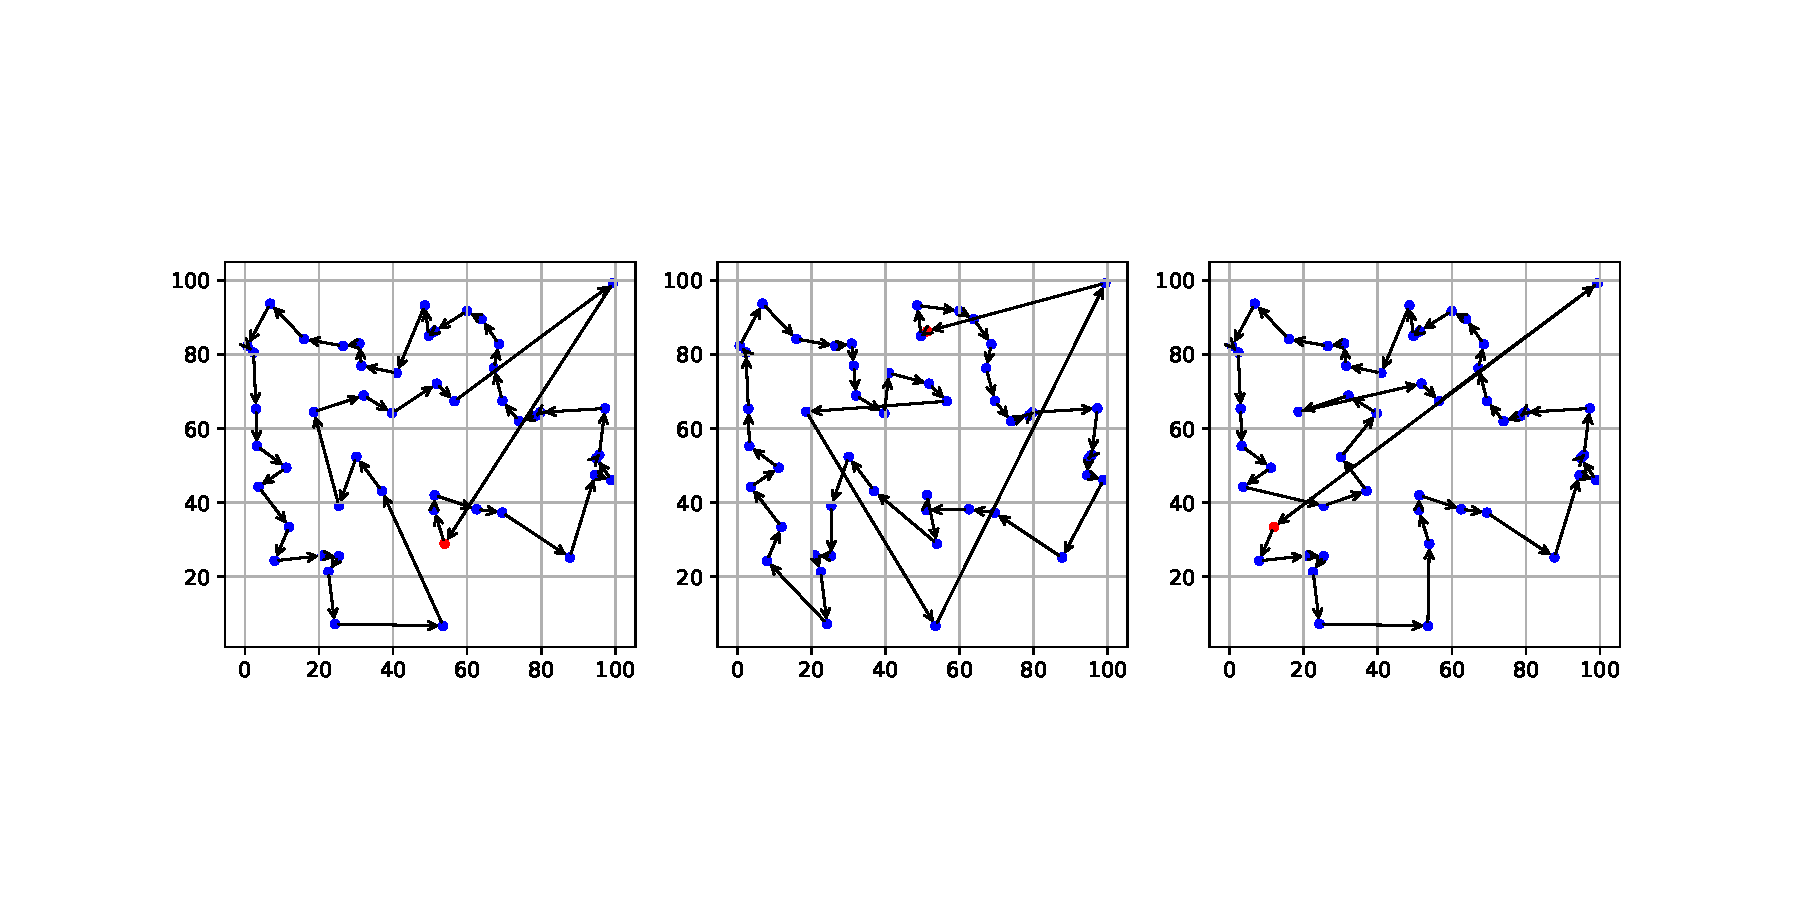
\includegraphics[width=\textwidth]{images/NN_50_villes_3departs.pdf}
    \caption{Résultat pour l'algorithme des Voisins plus proches avec trois départs différents (50 villes).}
    \label{fig:nn-50}
\end{figure}

\subsection*{2-opt}

\begin{figure}[H]
    \centering
    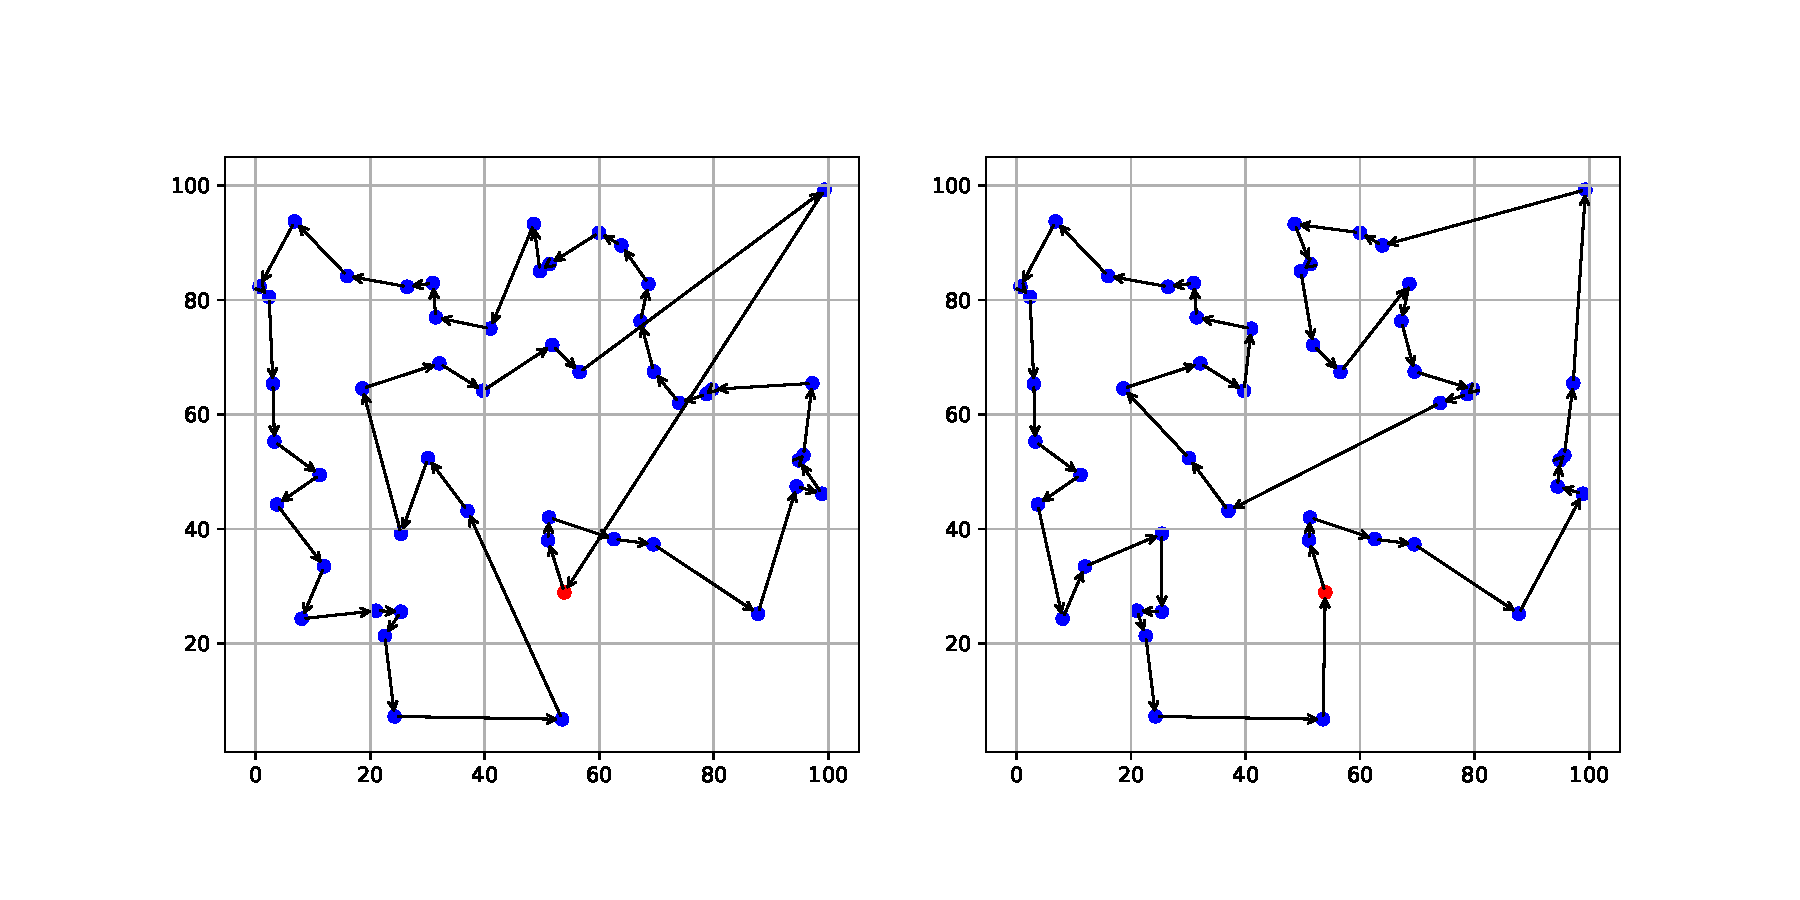
\includegraphics[width=\textwidth]{images/2opt_50_villes_nn.pdf}
    \caption{Résultat pour l'algorithme 2-opt et sa comparaison avec le résultat des Voisins plus proches (50 villes).}
    \label{fig:2opt-nn}
\end{figure}

\begin{figure}[H]
    \centering
    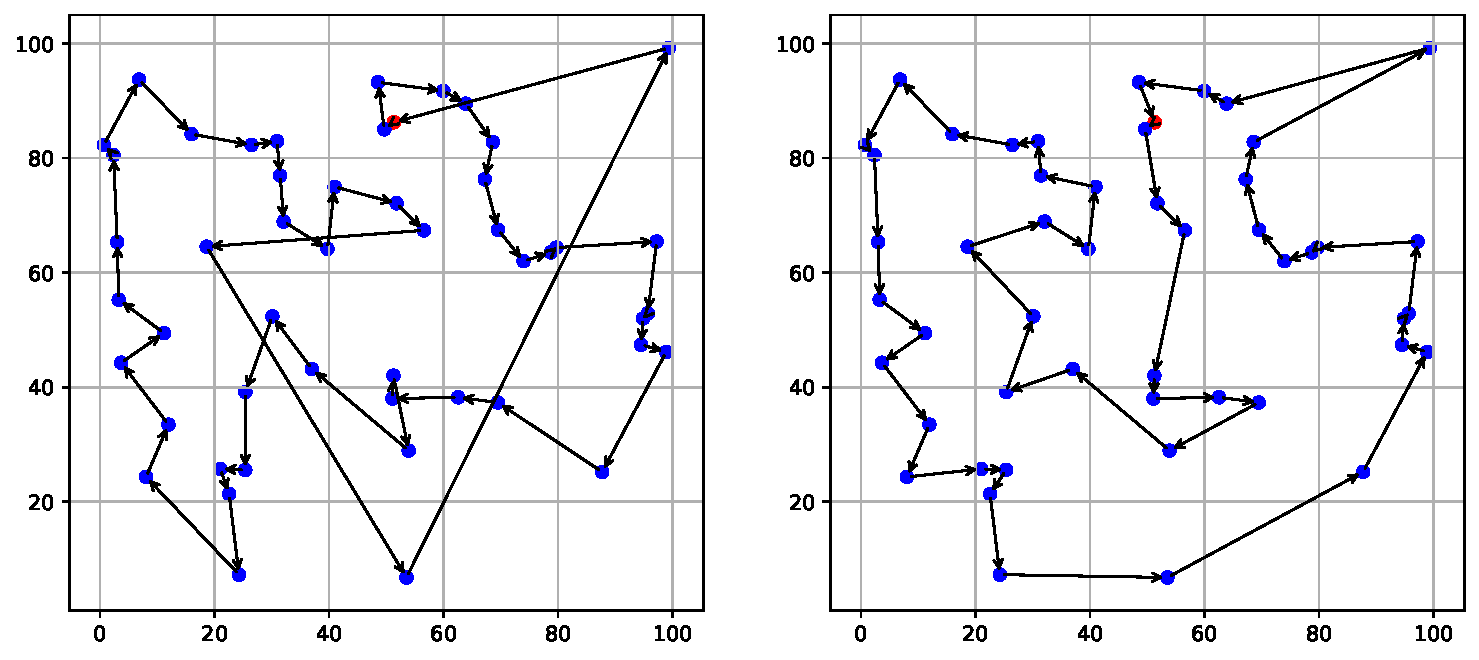
\includegraphics[width=\textwidth]{images/2opt_50_villes_depart_23.pdf}
    \caption{Résultat de 2-opt et sa comparaison avec le résultat des Voisins plus proches pour un départ au milieu.}
    \label{fig:2opt-dep23}
\end{figure}

\begin{figure}[H]
    \centering
    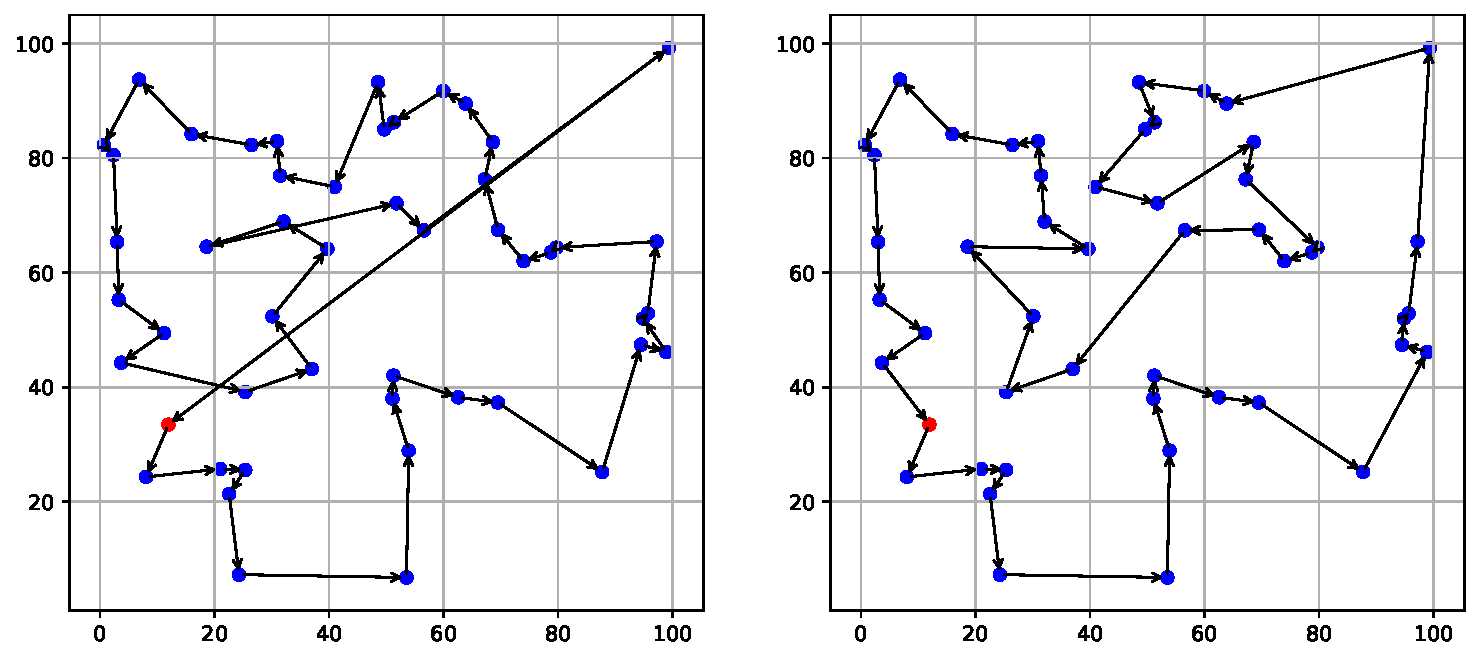
\includegraphics[width=\textwidth]{images/2opt_50_villes_depart_42.pdf}
    \caption{Résultat de 2-opt pour un départ différent. On vérifie que le résultat de 2-opt est dépendent du résultat initial des voisins plus proches, donc le résultat n'est pas fixé.}
    \label{fig:2opt-dep42}
\end{figure}

\subsection*{Heuristique d'insertion}
\paragraph{}
Pour l'heuristique d'insertion avec 20 villes, on obtient un graphe fluide avec une distance totale de 355.04 pour un temps de calcul de 0.000535 secondes.
\begin{figure}[H]
    \centering
    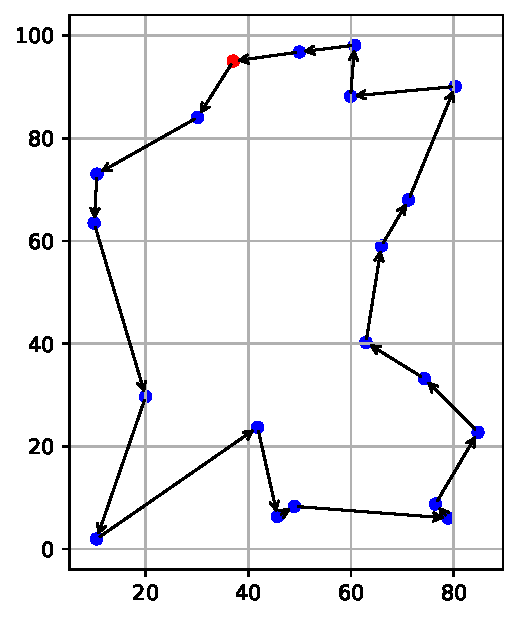
\includegraphics[width=0.35\textwidth]{images/insertion_20_villes.pdf}
    \caption{Résultat pour l'heuristique d'insertion avec 20 villes.}
    \label{fig:insert-20}
\end{figure}
\paragraph{}
Les résultats obtenus pour l'heuristique d'insertion avec 100 villes sont les suivants :
\begin{itemize}
    \item distance totale : 930.16
    \item temps de calcul : 0.024143 secondes
\end{itemize}
tandis que les résultats pour l'heuristique de voisins plus proches sont :
\begin{itemize}
    \item distance totale : 1062.79
    \item temps de calcul : 0.000609 secondes\\
Le second est certe plus rapide que le premier mais il est aussi un peu plus long, et comme on peut le voir sur la figure ci-après, l'heuristique d'insertion ne coupe pas le chemin contrairement au second ce qui le rend plus agréable à étudier. 
\end{itemize}
\begin{figure}[H]
    \centering
    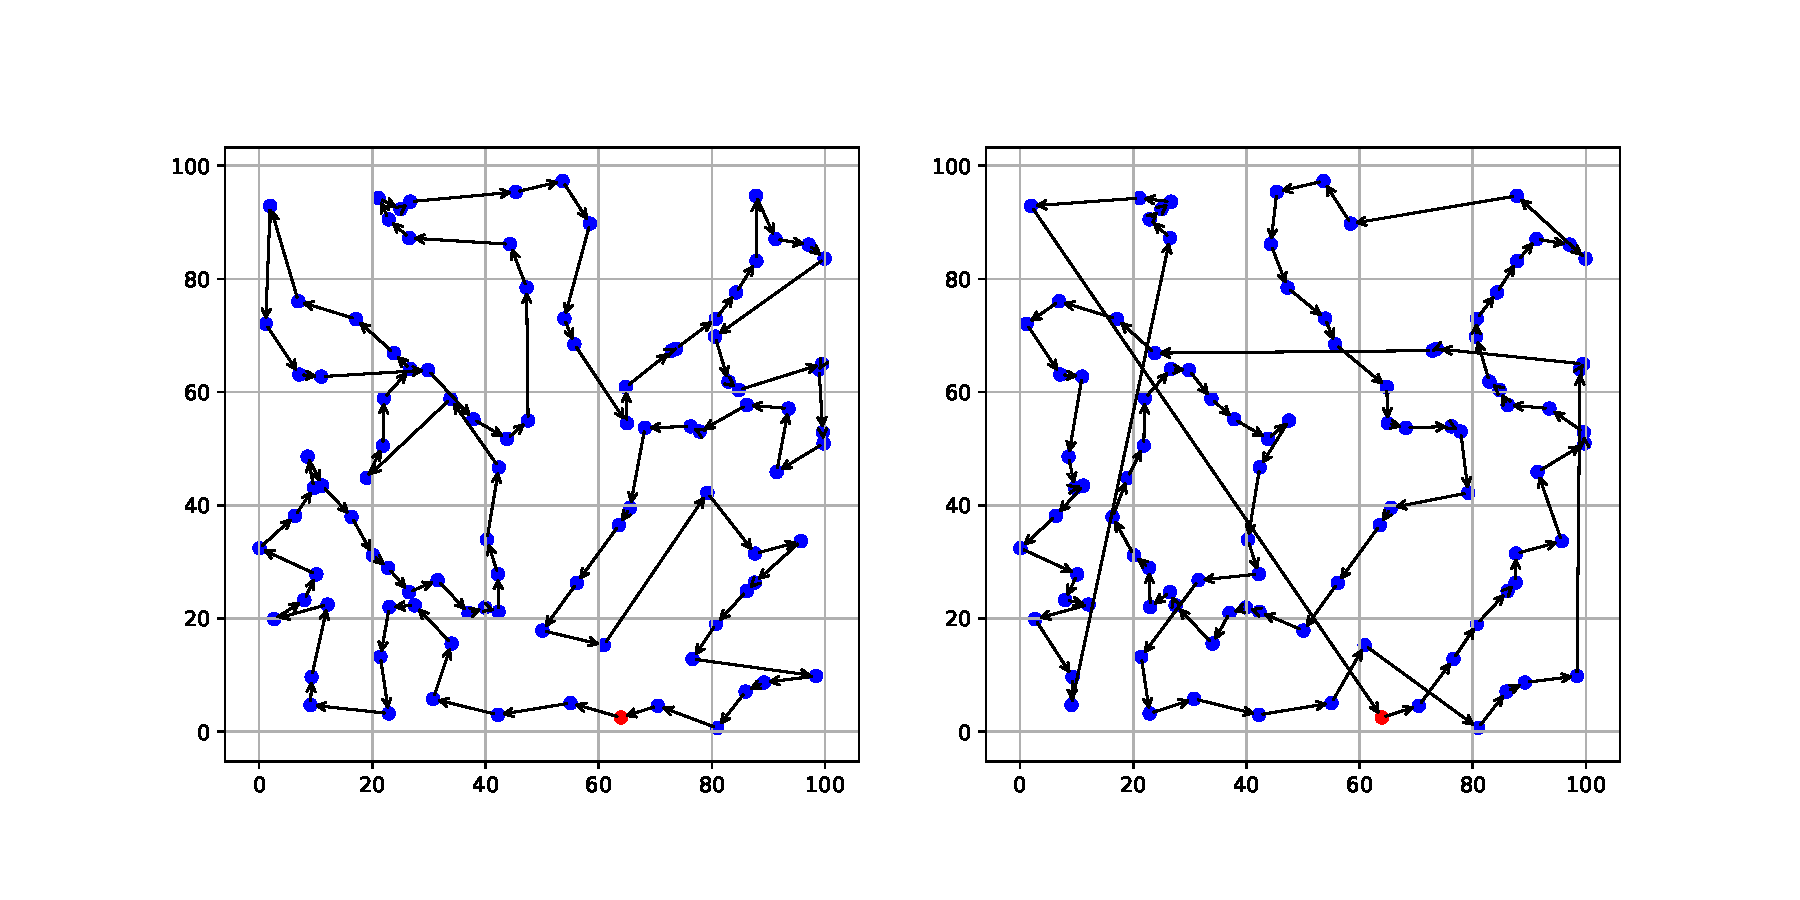
\includegraphics[width=\textwidth]{images/insertion_100_villes_nn.pdf}
    \caption{Résultat pour l'heuristique d'insertion avec 100 villes et une comparaison avec le résultat des Voisins plus proches pour le même réseau.}
    \label{fig:insert-100}
\end{figure}

\subsection*{Recuit simulé}
\paragraph{}
Nous obtenons les mesures suivantes : 
\begin{itemize}
    \item distance totale : 897.78
    \item temps de calcul : 0.031324
\end{itemize} 
pour l'heuristique d'insertion contre :
\begin{itemize}
    \item distance totale : 865.26
    \item temps de calcul : 0.308325 secondes
\end{itemize}
pour le recuit simule.
Comme on le constate sur la figure suivante, même si le temps de calcul augmente et est multiplié par 10 par rapport à l'heuristique d'insertion, la distance du chemin est diminuée. 
Le temps de calcul reste très faible : environ 0.3 secondes, ce qui rend le recuit simulé optimal pour des calculs de chemins avec un nombre de villes important.
\begin{figure}[H]
    \centering
    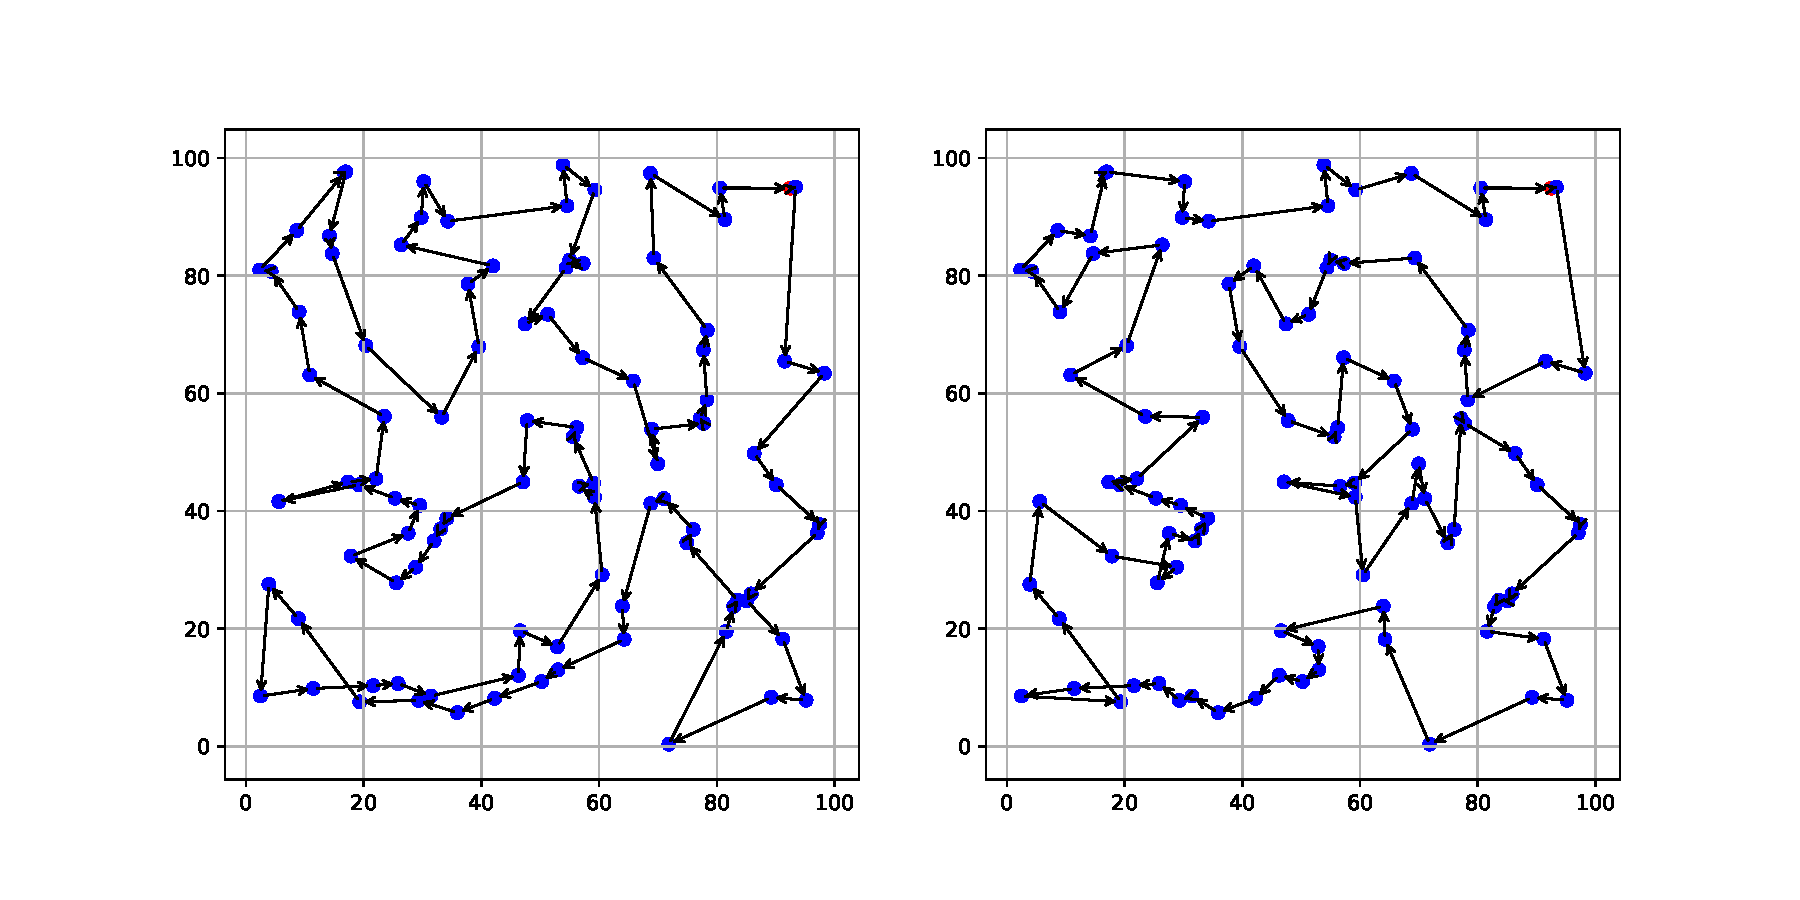
\includegraphics[width=\textwidth]{images/recuit_simule.pdf}
    \caption{Résultat pour l'heuristique d'insertion (à gauche) et sa amelioration par l'algorithme de Recuit simulé (à driote) avec 100 villes.}
    \label{fig:recuit}
\end{figure}

\subsection*{Comparaison et complexité}

\begin{table}[H]
    \centering
    \caption{Distance obtenu avec les différents algorithmes pour une quantité $N$ de villes.}
    \label{tab:distances}
    \begin{tabular}{lcccc}
        \hline
        N villes & VPP & 2-opt & Heuristique d'insertion & Recuit simulé \\ \hline\hline
        10  & 286.2587  & 266.1043  & 299.9325 & 266.1043 \\
        50  & 588.5159  & 549.2188  & 615.9452 & 565.7999 \\
        100 & 888.5622 & - & 853.6044 & 827.6085 \\
        500 & 2099.8537 & - & 1936.8251 & 1936.8251 \\
        1000 & 2916.9891 & - & 2716.844 & 2716.8443  \\ \hline
    \end{tabular}
\end{table}

\begin{figure}[H]
    \centering
    
\includegraphics[width=\textwidth]{images/complexite_temporelle.pdf}
    \caption{Nombre de villes vs. le temps moyenne d'execution des algorithmes.}
    \label{fig:temps}
\end{figure}

\newpage

\section*{\underline{Conclusion}}

\newpage
\bibliographystyle{unsrt}
\bibliography{bibliography}

\end{document}
